%%%%%%%%%%%%%%%%%%%%%%%%%%%%%%%%%%%%%%%%
% Main document for our awesome monography.
%
% Webpage:
% https://github.com/subleleks/monography
%%%%%%%%%%%%%%%%%%%%%%%%%%%%%%%%%%%%%%%%

% Computer Science Bachelor's Degree
\documentclass[bacharelado]{unb-cic}

%%%%%%%%%%%%%%%%%%%%%%%%%%%%%%%%%%%%%%%%
% Imported Packages
%
% Besides cute colors, we're using the
% portuguese version.
%%%%%%%%%%%%%%%%%%%%%%%%%%%%%%%%%%%%%%%%

\usepackage[brazil,american]{babel}
\usepackage[T1]{fontenc}
\usepackage{indentfirst}
\usepackage{natbib}
\usepackage{xcolor,graphicx,url}
\usepackage[utf8]{inputenc}

%%%%%%%%%%%%%%%%%%%%%%%%%%%%%%%%%%%%%%%%
% Cores dos links
%%%%%%%%%%%%%%%%%%%%%%%%%%%%%%%%%%%%%%%%

% Veja o arquivos cores.tex se quiser ver que outras cores estão
% pré-definidas.  Utilizando o comando \hypersetup abaixo nós
% evitamos aquelas caixas vermelhas feias em volta dos links.

%%%%%%%%%%%%%%%%%%%%%%%%%%%%%%%%%%%%%%%%
% Cores do estilo Tango
%%%%%%%%%%%%%%%%%%%%%%%%%%%%%%%%%%%%%%%%

\definecolor{LightButter}{rgb}{0.98,0.91,0.31}
\definecolor{LightOrange}{rgb}{0.98,0.68,0.24}
\definecolor{LightChocolate}{rgb}{0.91,0.72,0.43}
\definecolor{LightChameleon}{rgb}{0.54,0.88,0.20}
\definecolor{LightSkyBlue}{rgb}{0.45,0.62,0.81}
\definecolor{LightPlum}{rgb}{0.68,0.50,0.66}
\definecolor{LightScarletRed}{rgb}{0.93,0.16,0.16}
\definecolor{Butter}{rgb}{0.93,0.86,0.25}
\definecolor{Orange}{rgb}{0.96,0.47,0.00}
\definecolor{Chocolate}{rgb}{0.75,0.49,0.07}
\definecolor{Chameleon}{rgb}{0.45,0.82,0.09}
\definecolor{SkyBlue}{rgb}{0.20,0.39,0.64}
\definecolor{Plum}{rgb}{0.46,0.31,0.48}
\definecolor{ScarletRed}{rgb}{0.80,0.00,0.00}
\definecolor{DarkButter}{rgb}{0.77,0.62,0.00}
\definecolor{DarkOrange}{rgb}{0.80,0.36,0.00}
\definecolor{DarkChocolate}{rgb}{0.56,0.35,0.01}
\definecolor{DarkChameleon}{rgb}{0.30,0.60,0.02}
\definecolor{DarkSkyBlue}{rgb}{0.12,0.29,0.53}
\definecolor{DarkPlum}{rgb}{0.36,0.21,0.40}
\definecolor{DarkScarletRed}{rgb}{0.64,0.00,0.00}
\definecolor{Aluminium1}{rgb}{0.93,0.93,0.92}
\definecolor{Aluminium2}{rgb}{0.82,0.84,0.81}
\definecolor{Aluminium3}{rgb}{0.73,0.74,0.71}
\definecolor{Aluminium4}{rgb}{0.53,0.54,0.52}
\definecolor{Aluminium5}{rgb}{0.33,0.34,0.32}
\definecolor{Aluminium6}{rgb}{0.18,0.20,0.21}

\hypersetup{
  colorlinks=true,
  linkcolor=DarkOrange,
  citecolor=DarkOrange,
  filecolor=DarkOrange,
  urlcolor= DarkOrange
}


%%%%%%%%%%%%%%%%%%%%%%%%%%%%%%%%%%%%%%%%
% Monography Info
%%%%%%%%%%%%%%%%%%%%%%%%%%%%%%%%%%%%%%%%

\title{Um sistema computacional completo sobre uma máquina de instrução única implementada em FPGA}

\orientador{\prof \dr Marcus Vinicius Lamar}{CIC/UnB}
\coorientador{\prof \dr Diego de Freitas Aranha}{CIC/Unicamp}
\coordenador{\prof \dr Coordenador}{CIC/UnB}
\diamesano{30}{março}{2014}

\membrobanca{\prof \dr Professor I}{CIC/UnB}
\membrobanca{\prof \dr Professor II}{CIC/UnB}

\autor{Alexandre Silva}{Dantas}
\coautor{Matheus Costa de Sousa Carvalho}{Pimenta}
\CDU{004.4}

\palavraschave{palvrachave1, palvrachave2, palvrachave3 }
\keywords{keyword1, keyword2, keyword3}

%%%%%%%%%%%%%%%%%%%%%%%%%%%%%%%%%%%%%%%%
% Texto
%%%%%%%%%%%%%%%%%%%%%%%%%%%%%%%%%%%%%%%%

\begin{document}
  \maketitle
  \pretextual

  \begin{dedicatoria}
  Dedico a....\textbf{mamãe}
  \end{dedicatoria}

  \begin{agradecimentos}
  Agradeço a....\textit{papai}
  \end{agradecimentos}

  \begin{resumo}
  A ciência...
  \end{resumo}

  \selectlanguage{american}
  \begin{abstract}
  The science...
  \end{abstract}
  \selectlanguage{brazil}

  \tableofcontents
  \listoffigures
  \listoftables

  \textual
  
\chapter{Introdução}

Com a necessidade humana de se comunicar à distância, a engenharia deu luz às Telecomunicações (uma ref. aqui). Com esta novidade, é possível tanto que pais e filhos se comuniquem estando em cidades distintas, quanto estratégias de guerra sejam elaboradas em conjunto por países de continentes diferentes. Comum em ambas as situações, é o fato de que as duas pontas da comunicação desejam privacidade. Isto é, pais e filhos não querem que seus vizinhos tomem conhecimento das mensagens que trocam. Tampouco, países aliados pretendem que suas estratégias falhem por vazamento de informação.

Para tornar possível o sigilo na troca de mensagens à distância, estudos são realizados na área que hoje chamamos de Segurança da Informação (uma ref. aqui). Diversas técnicas são desenvolvidas nesta área até hoje, para tentar garantir que um par de comunicação possa trocar informações sem que estas chegem ao conhecimento de adversários. Entre estas técnicas, as mais conhecidas e utilizadas nasceram da Criptografia (uma ref. aqui).

A Criptografia estuda maneiras de criar uma versão ilegível de uma determinada mensagem, de modo que adversários com acesso ao canal inseguro pelo qual a mensagem será transmitida, por exemplo a Internet (uma ref. aqui), não tenham acesso à informação contida na mensagem, e de modo que somente o destinatário seja capaz de reverter este processo, que chamamos de cifragem. A Criptografia estuda também maneiras de autenticar uma fonte, isto é, um destinatário que recebe uma mensagem deve poder estar seguro de que esta foi de fato enviada pelo remetente do qual este destinatário espera receber esta mensagem.

Atualmente, os sistemas criptográficos mais empregados são os sistemas assimétricos (uma ref. aqui). Nestes sistemas, cada ponta da comunicação possui um par do que chamamos de chaves criptográficas. Uma chave criptográfica pode ser, por exemplo, uma frase. Os pares de chaves criptográficas são utilizados para cifrar e decifrar mensagens através de algoritmos criptográficos. Um algoritmo de criptografia assimétrica é uma sequência de passos que utiliza uma mensagem e uma chave de um par de chaves criptográficas para produzir algo que chamamos de criptograma, uma versão ilegível da mensagem original. Para reconstruir a mensagem original, utiliza-se uma sequência de passos de volta do algoritmo criptográfico, que utiliza o criptograma gerado anteriormente e a outra chave do par de chaves criptográficas. Sistemas criptográficos assimétricos utilizam pares de chaves, para que uma das chaves de alguém que se comunica seja pública, ou seja, conhecida por todos os que se comunicam, enquanto a outra chave do par deve ser privada, ou seja, somente este alguém que se comunica conhece sua chave privada. Deste modo, é possível trocar mensagens de maneira segura e simultaneamente autêntica, seguindo por exemplo a convenção de "assinar e colocar em um envelope" (cria-se um criptograma com a chave privada do remetente, une-se este criptograma com a mensagem original em uma única mensagem e transmite-se um criptograma da mensagem total, criado com a chave pública do destinatário. Deste modo, só o destinatário é capaz de abrir a mensagem total. Além disso, para verificar a autenticidade, basta verificar se a decifragem do criptograma interno utilizando a chave pública do remetente bate com a mensagem original).

É claro que entre os adversários interessados em obter informações sigilosas existem os mais astutos, praticantes de Criptanálise (uma ref. aqui). Diversas maneiras de se quebrar uma segurança são descobertas todos os dias. Uma maneira que vem sendo utilizada mais recentemente, devido ao aumento do poder computacional disponível, é a busca exaustiva por chaves (uma ref. aqui). É normal determinar que um sistema criptográfico é seguro se o melhor ataque conhecido não é mais eficiente do que a busca exaustiva no espaço de chaves.

Dos tipos de ataque existentes, o que é abordado neste trabalho chamamos de ataque de canal lateral (uma ref. aqui). Um ataque de canal lateral se baseia nas informações fornecidas pela parte física do sistema computacional utilizado para executar um algoritmo criptográfico, como por exemplo o consumo de energia em função do tempo.

Um computador funciona através de instruções. Uma instrução é um código que contém a informação de qual operação deve ser realiza pela máquina e quais dados devem ser utilizados como operandos. Historicamente, os primeiros computadores desenvolvidos são hoje chamados de computadores \textit{CISC} - \textit{Complex Instruction Set Computer}, ou Computador de Conjunto de Instruções Complexo (uma ref. aqui). O nome vem do fato de que os computadores oferenciam uma grande variedade de instruções, com diversas funcionalides complexas e por isso a estrutura interna da unidade central de processamento - \textit{CPU} - era bastante irregular, ou desorganizada.

Passado um certo tempo após a invenção dos processadores digitais, um novo modelo de arquitetura foi proposto. O modelo \textit{RISC} - \textit{Reduced Instruction Set Computer}, ou Computador de Conjunto de Instruções Reduzido (uma ref. aqui) - prega que o conjunto de instruções de um computador deve ser regular, de modo que é possível otimizar as operações mais frequentes na implementação da \textit{CPU}.

Sabe-se que a intensidade do consumo de energia de um processador digital, em um determinado instante do tempo, depende diretamente da instrução que está sendo executada (uma ref. aqui). Em um computador \textit{CISC} isto é mais evidente, dado que a irregularidade do conjunto de instruções se reflete na implementação física do processador. Em contrapartida, é de se esperar que computadores \textit{RISC} reflitam consumos de energia por instrução mais ininteligíveis. No entanto, os consumos de energia por instrução em computadores \textit{RISC} não são indiferenciáveis ao ponto de que um atacante experiente seja impedido de identificar um algoritmo criptográfico que está sendo executado em uma máquina deste tipo.

Mais recentemente, surgiu o modelo de computador \textit{OISC} - \textit{One Instruction Set Computer}, ou Computador de Instrução Única (uma ref. aqui). Computadores \textit{OISC} possuem a vantagem de que, independente do consumo de energia em função do tempo, não é possível diferenciar quais instruções estão sendo executadas em um intervalo de tempo, porque só existe uma única instrução! A tendência do consumo de energia de uma \textit{CPU} \textit{OISC} em função do tempo é ser uma função periódica, isto é, uma função cujo valor em qualquer ponto inicial é exatamente o mesmo que o avaliado em qualquer ponto cuja distância ao ponto inicial é um valor múltiplo de um determinado período (neste caso, um período de tempo). No entanto, por mais que hajam pequenas oscilações no consumo de energia, a dificuldade de se não poder identificar qual operação está sendo de fato executada em um determinado instante cria uma grande dificuldade para ataques de canal lateral.

Apesar de ser um modelo de computador mais seguro, computadores \textit{OISC} não são muito atraentes, por conta do fato de que quanto mais reduzido é o conjunto de instruções de um computador, mais trabalho é colocado sobre os ombros dos programadores. O objetivo deste trabalho, no entanto, é mostrar que é possível construir um sistema computacional completo, de propósito geral, sobre uma máquina de instrução única. O sistema foi construído em um \textit{FPGA} - \textit{Field-programmable Gate Array}, ou Arranjo de Portas Programável em Campo (uma ref. aqui) - utilizando a instrução Turing-completa \textit{subleq} - \textit{Subtract and branch if less or equal to zero}, ou subtrair e pular para outra instrução se o resultado for menor ou igual a zero (uma ref. aqui).

O sistema computacional aqui proposto contempla todos os níveis de abstração de um sistema computacional. Indo do nível mais baixo ao mais alto, implementamos o \textit{hardware} (incluindo \textit{CPU} e controladores de dispositivos externos), o \textit{software} básico (incluindo compilador, montador, ligador e sistema operacional) e \textit{softwares} de aplicação (incluindo aplicações com algoritmos criptográficos).

  \chapter{Protótipo do Segundo Capítulo}

\section{Conceitos Básicos}

% Começando do básico do básico do básico

Computadores são sistemas incrivelmente complexos. Inúmeros componentes com
papeis específicos necessitam de se intercomunicar para executar a mais simples das
tarefas. Dessa forma, para compreender seu funcionamento, se faz o uso de
camadas de abstrações.

% Camadas de abstrações
Essas camadas exercem funções diferentes e são visíveis de acordo com seu uso
--- um usuário final não precisa saber programar para usar um processador de
texto; da mesma forma, um programador não necessita saber da estrutura dos
circuitos internos. Cada camada possui seu domínio, sendo as mais próximas do
usuário final denominadas de ``alto-nível'' e as mais próximas dos transistores
e fios, ``baixo-nível''. Observe a figura \ref{camadas}, especificada de acordo
com Murdocca \cite{principles}.

% As várias camadas bonitinhas
\begin{figure}[ptb]
  \begin{center}
    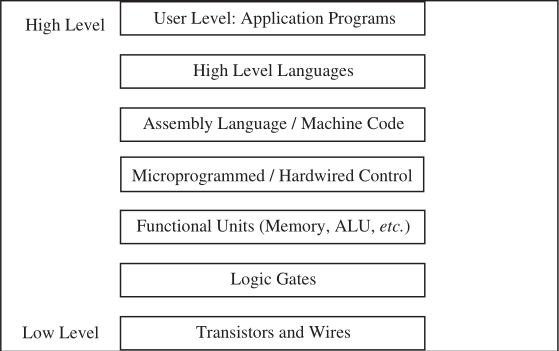
\includegraphics[scale=.6]{imagens/1_camadas}
  \end{center}
  \caption{Camadas de abstração de um computador.}
  \label{camadas}
\end{figure}

% Arquitetura do Computador -> ISA

Uma definição muito importante para o programador de sistema é a Arquitetura do
Conjunto de Instruções (\textit{Instruction Set Arquitecture}) --- de agora em
diante referida apenas como arquitetura, ou \textit{ISA}. Hennessy a define como
``o limite entre \textit{software} e \textit{hardware}'' \cite{hennessy}.

% Componentes da ISA
% (devo definir o que é "programa de sistema"?)
A \textit{ISA} descreve vários componentes essenciais para a criação de
programas de sistema. Seu \textit{design} define a memória interna do
processador, o endereçamento de memória interna e externa, quais
instruções/operações são suportadas, tipos e tamanhos de operandos, dentre
muitos outros  \cite{patterson}.

Existem tipos diferentes de \textit{ISA}, sendo comuns as arquiteturas
\textit{RISC} e \textit{CISC}.

% ISA -> RISC e CISC
Arquiteturas \textit{RISC} (\textit{Reduced Instruction Set Computer}) possuem
uma quantidade reduzida de instruções. Em geral são instruções simples e rápidas
que têm de ser combinadas para ações mais complexas. Já arquiteturas
\textit{CISC} (\textit{Complex Instruction Set Computer}) provêem uma quantidade
maior de instruções, que nativamente executam ações mais complicadas e
abrangentes.

% Vantagens da RISC
Instruções da arquitetura \textit{RISC} são mais simples; elas partem da
filosofia de otimizar os casos frequentes, visando tornar o comportamento geral
mais rápido. Murdocca argumenta que um conjunto de instruções mais simples
resulta numa central de processamento simples e menor, liberando espaço no
processador para outros componentes, como registradores \cite{principles}.

% Desvantagens da RISC
Porém Mostafa argumenta que isso traz a desvantagem de que uma grande quantidade
de instruções são necessárias para executar uma função simples \cite{mostafa},
possivelmente reduzindo o desempenho geral. Por fim, isso tambem causa um
problema cognitivo, já que programas \textit{RISC} tendem a ser mais verbosos e
depositarem a complexidade do programa nos ombros do programador.

% OISC
Além de ambas as \textit{ISA}s citadas acima, existe a arquitetura \textit{OISC}
(\textit{One Instruction Set Computer}). Ela define computadores com apenas uma
única instrução. De acordo com Gilreath, \textit{OISC} é como um \textit{CISC}
em um nível mais alto de abstração, já que precisa-se combinar essa única
instrução de diversas formas para sintetizar o que seriam as instruções mais
complexas \cite{minimalist}.

% Será que eu devo falar sobre coisas Turing-completas?
% Como OISC são equivalentes às RISC/CISC nesse sentido?

% Mesmas desvantagens de RISC
Pela própria definição, arquiteturas \textit{OISC} possuem as desvantagens de
\textit{RISC} em escala muito maior. Qualquer função simples necessitará de
várias combinações da única instrução, dificultando tanto a velocidade quanto
compreensão do programa final.

Entretanto, existem vantagens na previsibilidade de máquinas \textit{OISC}.

% Dar introdução à criptografia?

% CISC/RISC, gasto de energia diferente
Em máquinas não-\textit{OISC}, existe um conjunto bem-definido de instruções que
podem ser executadas. Cada uma exige demandas específicas do processador,
resultando em gastos de energia possivelmente diferentes.

% Olhando o gasto de energia, deduzir instruções.
% (CITAÇÃO AQUI?)
Dessa forma, ao se monitorar o gasto de energia por um período suficiente de
tempo, pode-se observar os padrões de gasto de energia do processador. Então, um
observador externo poderá deduzir quais instruções foram executadas na máquina
sem necessariamente ter acesso à mesma.

Considerando que arquiteturas \textit{OISC} possuem apenas uma instrução, cuja
demanda ao processador é única, assume-se que o gasto de energia será
constante. Logo, não seria possível determinar quais ações essa máquina executou
independentemente da quantidade de tempo de monitoramento.

% Gasto de energia deve ser constante
O ponto abordado nesse trabalho é exatamente esse --- determinar se o gasto de
energia em função do tempo é constante numa máquina \textit{OISC}. Se for o
caso, pode-se determinar aplicações interessantes para esse tipo de computador
na área de segurança de informação e criptografia.

Primeiramente, devemos determinar que instrução será usada na nossa máquina
\textit{OISC}.

\section{Linguagem de Montagem Subleq}
\label{sec:subleq}

Existem várias máquinas de arquitetura \textit{OISC}. Uma delas é a máquina que
possui apenas a instrução \textit{SUBLEQ} (\textit{Subtract and Branch on Less
  or Equal} \cite{subleq}.

% Pontos positivos
% * Previsibilidade
% Pontos negativos
% * Impacto na velocidade de execução


  \chapter{Revisão Bibliográfica}

  \chapter{Metodologia}

  \chapter{Protótipo do Quinto Capítulo}

\section{Conceitos Básicos}

% Começando do básico do básico do básico

Computadores são sistemas incrivelmente complexos. Inúmeros componentes com
papeis específicos necessitam de se intercomunicar para executar a mais simples das
tarefas. Dessa forma, para compreender seu funcionamento, se faz o uso de
camadas de abstrações.

% Camadas de abstrações
Essas camadas exercem funções diferentes e são visíveis de acordo com seu uso
--- um usuário final não precisa saber programar para usar um processador de
texto; da mesma forma, um programador não necessita saber da estrutura dos
circuitos internos. Cada camada possui seu domínio, sendo as mais próximas do
usuário final denominadas de ``alto-nível'' e as mais próximas dos transistores
e fios, ``baixo-nível''. Observe a figura \ref{camadas}, especificada de acordo
com Murdocca \cite{principles}.

% As várias camadas bonitinhas
\begin{figure}[ptb]
  \begin{center}
    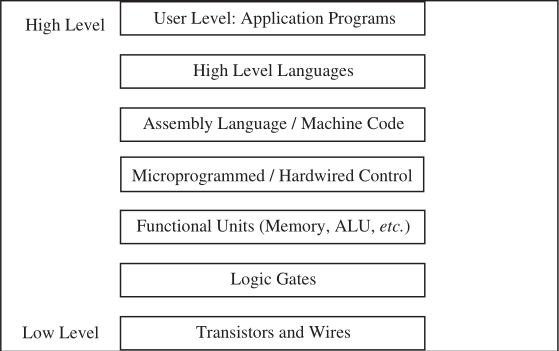
\includegraphics[scale=.6]{imagens/1_camadas}
  \end{center}
  \caption{Camadas de abstração de um computador.}
  \label{camadas}
\end{figure}

% Arquitetura do Computador -> ISA

Uma definição muito importante para o programador de sistema é a Arquitetura do
Conjunto de Instruções (\textit{Instruction Set Arquitecture}) --- de agora em
diante referida apenas como arquitetura, ou \textit{ISA}. Hennessy a define como
``o limite entre \textit{software} e \textit{hardware}'' \cite{hennessy}.

% Componentes da ISA
% (devo definir o que é "programa de sistema"?)
A \textit{ISA} descreve vários componentes essenciais para a criação de
programas de sistema. Seu \textit{design} define a memória interna do
processador, o endereçamento de memória interna e externa, quais
instruções/operações são suportadas, tipos e tamanhos de operandos, dentre
muitos outros  \cite{patterson}.

Existem tipos diferentes de \textit{ISA}, sendo comuns as arquiteturas
\textit{RISC} e \textit{CISC}.

% ISA -> RISC e CISC
Arquiteturas \textit{RISC} (\textit{Reduced Instruction Set Computer}) possuem
uma quantidade reduzida de instruções. Em geral são instruções simples e rápidas
que têm de ser combinadas para ações mais complexas. Já arquiteturas
\textit{CISC} (\textit{Complex Instruction Set Computer}) provêem uma quantidade
maior de instruções, que nativamente executam ações mais complicadas e
abrangentes.

% Vantagens da RISC
Instruções da arquitetura \textit{RISC} são mais simples; elas partem da
filosofia de otimizar os casos frequentes, visando tornar o comportamento geral
mais rápido. Murdocca argumenta que um conjunto de instruções mais simples
resulta numa central de processamento simples e menor, liberando espaço no
processador para outros componentes, como registradores \cite{principles}.

% Desvantagens da RISC
Porém Mostafa argumenta que isso traz a desvantagem de que uma grande quantidade
de instruções são necessárias para executar uma função simples \cite{mostafa},
possivelmente reduzindo o desempenho geral. Por fim, isso tambem causa um
problema cognitivo, já que programas \textit{RISC} tendem a ser mais verbosos e
depositarem a complexidade do programa nos ombros do programador.

% OISC
Além de ambas as \textit{ISA}s citadas acima, existe a arquitetura \textit{OISC}
(\textit{One Instruction Set Computer}). Ela define computadores com apenas uma
única instrução. De acordo com Gilreath, \textit{OISC} é como um \textit{CISC}
em um nível mais alto de abstração, já que precisa-se combinar essa única
instrução de diversas formas para sintetizar o que seriam as instruções mais
complexas \cite{minimalist}.

% Será que eu devo falar sobre coisas Turing-completas?
% Como OISC são equivalentes às RISC/CISC nesse sentido?

% Mesmas desvantagens de RISC
Pela própria definição, arquiteturas \textit{OISC} possuem as desvantagens de
\textit{RISC} em escala muito maior. Qualquer função simples necessitará de
várias combinações da única instrução, dificultando tanto a velocidade quanto
compreensão do programa final.

Entretanto, existem vantagens na previsibilidade de máquinas \textit{OISC}.

% Dar introdução à criptografia?

% CISC/RISC, gasto de energia diferente
Em máquinas não-\textit{OISC}, existe um conjunto bem-definido de instruções que
podem ser executadas. Cada uma exige demandas específicas do processador,
resultando em gastos de energia possivelmente diferentes.

% Olhando o gasto de energia, deduzir instruções.
% (CITAÇÃO AQUI?)
Dessa forma, ao se monitorar o gasto de energia por um período suficiente de
tempo, pode-se observar os padrões de gasto de energia do processador. Então, um
observador externo poderá deduzir quais instruções foram executadas na máquina
sem necessariamente ter acesso à mesma.

Considerando que arquiteturas \textit{OISC} possuem apenas uma instrução, cuja
demanda ao processador é única, assume-se que o gasto de energia será
constante. Logo, não seria possível determinar quais ações essa máquina executou
independentemente da quantidade de tempo de monitoramento.

% Gasto de energia deve ser constante
O ponto abordado nesse trabalho é exatamente esse --- determinar se o gasto de
energia em função do tempo é constante numa máquina \textit{OISC}. Se for o
caso, pode-se determinar aplicações interessantes para esse tipo de computador
na área de segurança de informação e criptografia.

Primeiramente, devemos determinar que instrução será usada na nossa máquina
\textit{OISC}.

\section{Linguagem de Montagem Subleq}
\label{sec:subleq}

Existem várias máquinas de arquitetura \textit{OISC}. Uma delas é a máquina que
possui apenas a instrução \textit{SUBLEQ} (\textit{Subtract and Branch on Less
  or Equal} \cite{subleq}.

% Pontos positivos
% * Previsibilidade
% Pontos negativos
% * Impacto na velocidade de execução


  % ...

  \postextual
  \bibliographystyle{plain}
  \bibliography{bibliografia}

\end{document}
